\documentclass[12pt]{article}
\usepackage[utf8]{inputenc}
\usepackage[spanish,es-lcroman, es-tabla]{babel}
\usepackage[autostyle,spanish=mexican]{csquotes}
\usepackage{amsmath}
\usepackage{amssymb}
\usepackage{nccmath}
\numberwithin{equation}{section}
\usepackage{amsthm}
\usepackage{graphicx}
\usepackage{epstopdf}
\DeclareGraphicsExtensions{.pdf,.png,.jpg,.eps}
\usepackage{color}
\usepackage{float}
\usepackage{multicol}
\usepackage{enumerate}
\usepackage[shortlabels]{enumitem}
\usepackage{anyfontsize}
\usepackage{anysize}
\usepackage{array}
\usepackage{multirow}
\usepackage{enumitem}
\usepackage{cancel}
\usepackage{tikz}
\usepackage{circuitikz}
\usepackage{tikz-3dplot}
\usetikzlibrary{babel}
\usepackage{bm}
\usepackage{mathtools}
\usepackage{esvect}
\usepackage{hyperref}
\usepackage{relsize}
\usepackage{siunitx}
\usepackage{physics}
%\usepackage{biblatex}
\usepackage{standalone}
\usepackage{mathrsfs}
\usepackage{bigints}
\usepackage{bookmark}
\spanishdecimal{.}

\setlist[enumerate]{itemsep=0mm}

\renewcommand{\baselinestretch}{1.5}

\let\oldbibliography\thebibliography

\renewcommand{\thebibliography}[1]{\oldbibliography{#1}

\setlength{\itemsep}{0pt}}
%\marginsize{1.5cm}{1.5cm}{2cm}{2cm}


\newtheorem{defi}{{\it Definición}}[section]
\newtheorem{teo}{{\it Teorema}}[section]
\newtheorem{ejemplo}{{\it Ejemplo}}[section]
\newtheorem{propiedad}{{\it Propiedad}}[section]
\newtheorem{lema}{{\it Lema}}[section]

\setlength{\jot}{12pt}
\title{Funciones generadas a partir de la ED de Bessel \\ {\large Tema 5 - Matemáticas Avanzadas de la Física}\vspace{-1.5\baselineskip}}
\author{}
\date{}
\begin{document}
\maketitle
\fontsize{14}{14}\selectfont
\begin{table}[H]
%{\setlength\extrarowheight{0.5pt}
{\renewcommand{\arraystretch}{1.75}%
\begin{threeparttable}
\begin{tabular}{p{6cm} l}
Funciones de Bessel & $J_{n}(x) = \sum_{s=0}^{\infty} \dfrac{(-1)^{s}}{s!\, (n + s)!} \, \left( \dfrac{x}{2} \right)^{n+2s}$ \\ \hline
Funciones de Neumann & $N_{\nu} (x) = \dfrac{J_{\nu}(x) \, \cos \nu \pi - J_{-\nu}(x)}{\sin \nu \pi}$ \\ \hline
\multirow{2}{*}{Funciones de Hankel\tnote{1}} & $ H_{\nu}^{(1)} (x) = J_{\nu} (x) + N_{\nu}(x)$ \\
& $ H_{\nu}^{(2)} (x) = J_{\nu} (x) - N_{\nu}(x)$ \\ \hline
\multirow{2}{*}{Funciones modificadas de Bessel\tnote{2}} & $I_{\nu}(x) = e^{-\nu \pi i /2} \, J_{\nu} (x \, e^{i \pi 2})$ \\
 & $K_{\nu} (x) = \dfrac{2}{\pi} \, \dfrac{I_{-\nu}(x) - I_{\nu} (x)}{\sin \nu \pi}$ \\ \hline
 \multirow{4}{*}{Funciones esféricas de Bessel\tnote{3}} & $j_{n} (x) = \sqrt{\dfrac{\pi}{2 x}} \, J_{n+\frac{1}{2}} (x)$ \\
 & $n_{n} (x) = \sqrt{\dfrac{\pi}{2 x}} \, N_{n+\frac{1}{2}} (x) = (-1)^{n+1} \sqrt{\dfrac{\pi}{2 x}} J_{-n-\frac{1}{2}} (x)$ \\
 & $h_{n}^{(1)} (x) = \sqrt{\dfrac{\pi}{2 x}} \, H_{n+\frac{1}{2}}^{(1)} (x) = j_{n}(x) + i \, n_{n} (x)$ \\
 & $h_{n}^{(2)} (x) = \sqrt{\dfrac{\pi}{2 x}} \, H_{n+\frac{1}{2}}^{(2)} (x) = j_{n}(x) - i \, n_{n} (x)$ \\ \hline
\end{tabular}
\begin{tablenotes}
\item[1] \footnotesize Las funciones de Hankel se utilizan para representar las soluciones de ondas entrantes y salientes de una ecuación de ondas bajo simetría cilíndrica respectivamente (o viceversa, dependiendo de la convención del signo de la frecuencia). 
\item[2] Las funciones de Bessel ordinarias son válidas para valores complejos del argumento $x$, y un caso especialmente importante es aquel con argumento imaginario puro, dando origen a las funciones modificadas de Bessel.
\item[3] Cuando se resuelve la ecuación de Helmholtz en coordenadas esféricas mediante la técnica de separación de variables, las soluciones a la ecuación radial son las funciones esféricas de Bessel.
\end{tablenotes}
\end{threeparttable}}
\end{table}
%\newpage
\newgeometry{left=1cm,right=1cm, top=1.5cm, bottom=1.5cm}
Las siguientes gráficas se generaron utilizando: a) la librería \texttt{scipy.special}, b) la librería de visualización \texttt{matplotlib}, ambas librerías de \texttt{python}.

\begin{figure}[H]
    \centering
    \begin{minipage}{0.4\linewidth}
        \includegraphics[scale=0.6]{Imagenes/plot_bessel.eps}
    \end{minipage}
    \hspace{1cm}
    \begin{minipage}{0.4\linewidth}
        \includegraphics[scale=0.6]{Imagenes/plot_neumann.eps}
    \end{minipage}
\end{figure}
\begin{figure}[H]
    \centering
    \begin{minipage}{0.4\linewidth}
        \includegraphics[scale=0.6]{Imagenes/plot_Modificadas_Bessel_01.eps}
    \end{minipage}
    \hspace{1cm}
    \begin{minipage}{0.4\linewidth}
        \includegraphics[scale=0.6]{Imagenes/plot_Modificadas_Bessel_02.eps}
    \end{minipage}
\end{figure}
\begin{figure}[H]
    \centering
    \begin{minipage}{0.4\linewidth}
        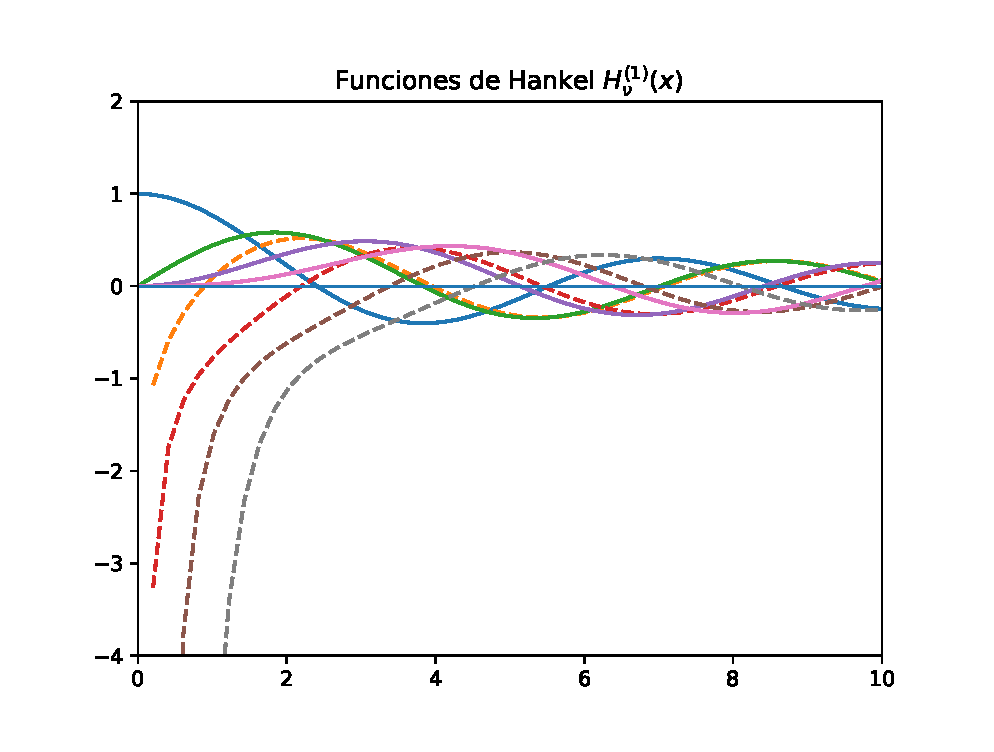
\includegraphics[scale=0.6]{Imagenes/plot_Hankel_01.eps}
    \end{minipage}
    \hspace{1cm}
    \begin{minipage}{0.4\linewidth}
        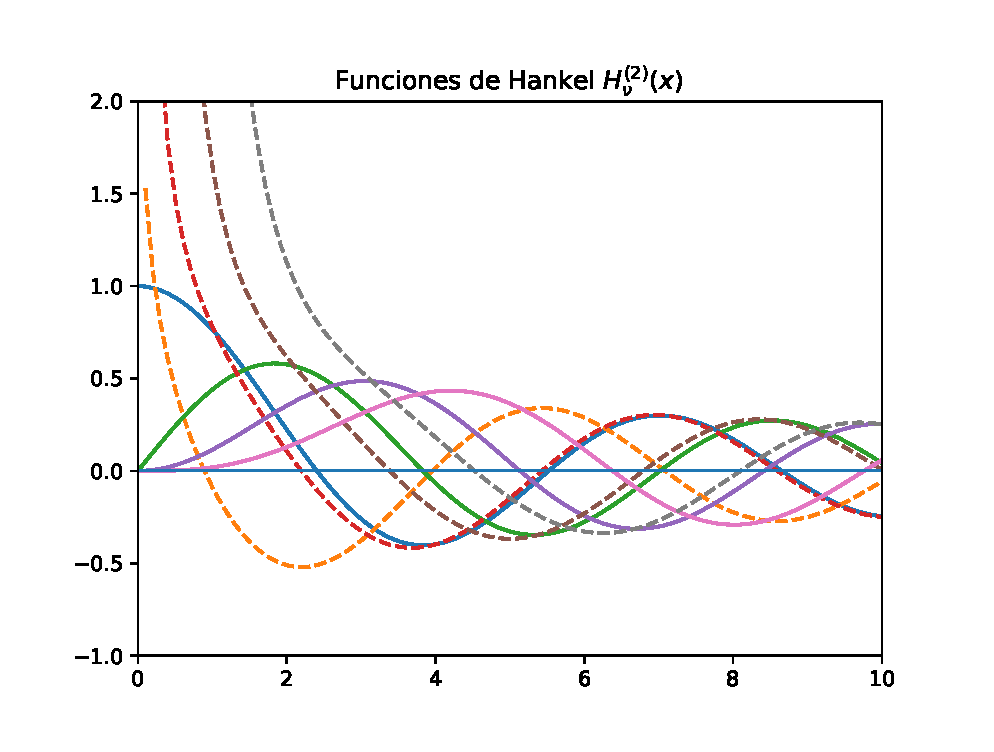
\includegraphics[scale=0.6]{Imagenes/plot_Hankel_02.eps}
    \end{minipage}
\end{figure}
\end{document}